\documentclass[a4paper,12pt]{article}
\usepackage{czech}
\usepackage[utf8]{inputenc}
\usepackage{a4wide}
\usepackage[dvipdfm]{graphicx}
\usepackage{indentfirst}
\usepackage{fancyhdr}
\usepackage{setspace}
\usepackage{amsmath}
\usepackage{amssymb}
\usepackage{epsfig}

%%\usepackage{nopageno}
%%\usepackage{txfonts}
\usepackage[usenames]{color}

\begin{document}
\section{Úkol}
\noindent
\begin{enumerate}
    \item Pomocí osciloskopu změřte špičkovou hodnotu napětí na sekundáru převodního transformátoru a porovnejte ji s hodnotou naměřenou voltmetrem.
    \item Podle vlastní volby sledujte činnost jednocestného nebo dvoucestného usměrňovače s křemíkovými diodami KY711
    \begin{enumerate}
        \item při maximální hodnotě zatěžovacího odporu 10 k$\Omega$ sledujte závislost stejnosměrného napětí na filtrační kapacitě $C$ v intervalu 0 – 10 $\mu$F. Hodnotu usměrněného napětí při $C = 10 \mu$F srovnejte se špičkovou hodnotou pulzního průběhu
        \item změřte závislost filtrační kapacity $C$, potřebné k tomu, aby střídavá složka usměrněného napětí tvořila 10\% špičkové hodnoty (tj. asi 1 V), na odebíraném proudu. U jednocestného usměrňovače měřte do proudu 0,6 mA, u dvoucestného do proudu 1 mA.
        \item naměřené závislosti zpracujte graficky. Do grafu uvádějícího závislost filtrační kapacity $C$ na proudu vyneste také závislost časové konstanty $\tau = R_zC$ na proudu. 
    \end{enumerate}
    \item Charakteristiku vakuové diody EZ81 a Zenerovy diody KZ703 zobrazte na osciloskopu podle schématu připojeného k úloze. Orientačně načrtněte pozorované charakteristiky a vyznačte měřítka na osách. Odhadněte napětí na diodách při proudu 20 mA v propustném směru. Určete Zenerovo napětí. 
\end{enumerate}

\section{Teorie}
\subsection{Efektivní hodnota}
Efektivní hodnota veličiny $A$ je dána vztahem
\begin{eqnarray}
A_e=\frac{1}{T}\int_0^TA(t)\mbox(d)t.
\end{eqnarray}
Pro periodicé veličiny, jako třeba napětí střídavého proudu, by tato hodnota byla nulová, proto pro její charakteristiku užívá
\begin{eqnarray}
U_e^2=\frac{1}{T}\int_0^Tu^2(t)\mbox{d}t,
\end{eqnarray}
což je pro speciálně pro sinový průběh
\begin{eqnarray}
U_e=\frac{U_0}{\sqrt{2}}.
\label{U_e}
\end{eqnarray}
Přesně tuto hodnotu nám ukazuje běžný voltmetr. Analogický vztah platí pro střídavý proud.

\begin{figure}
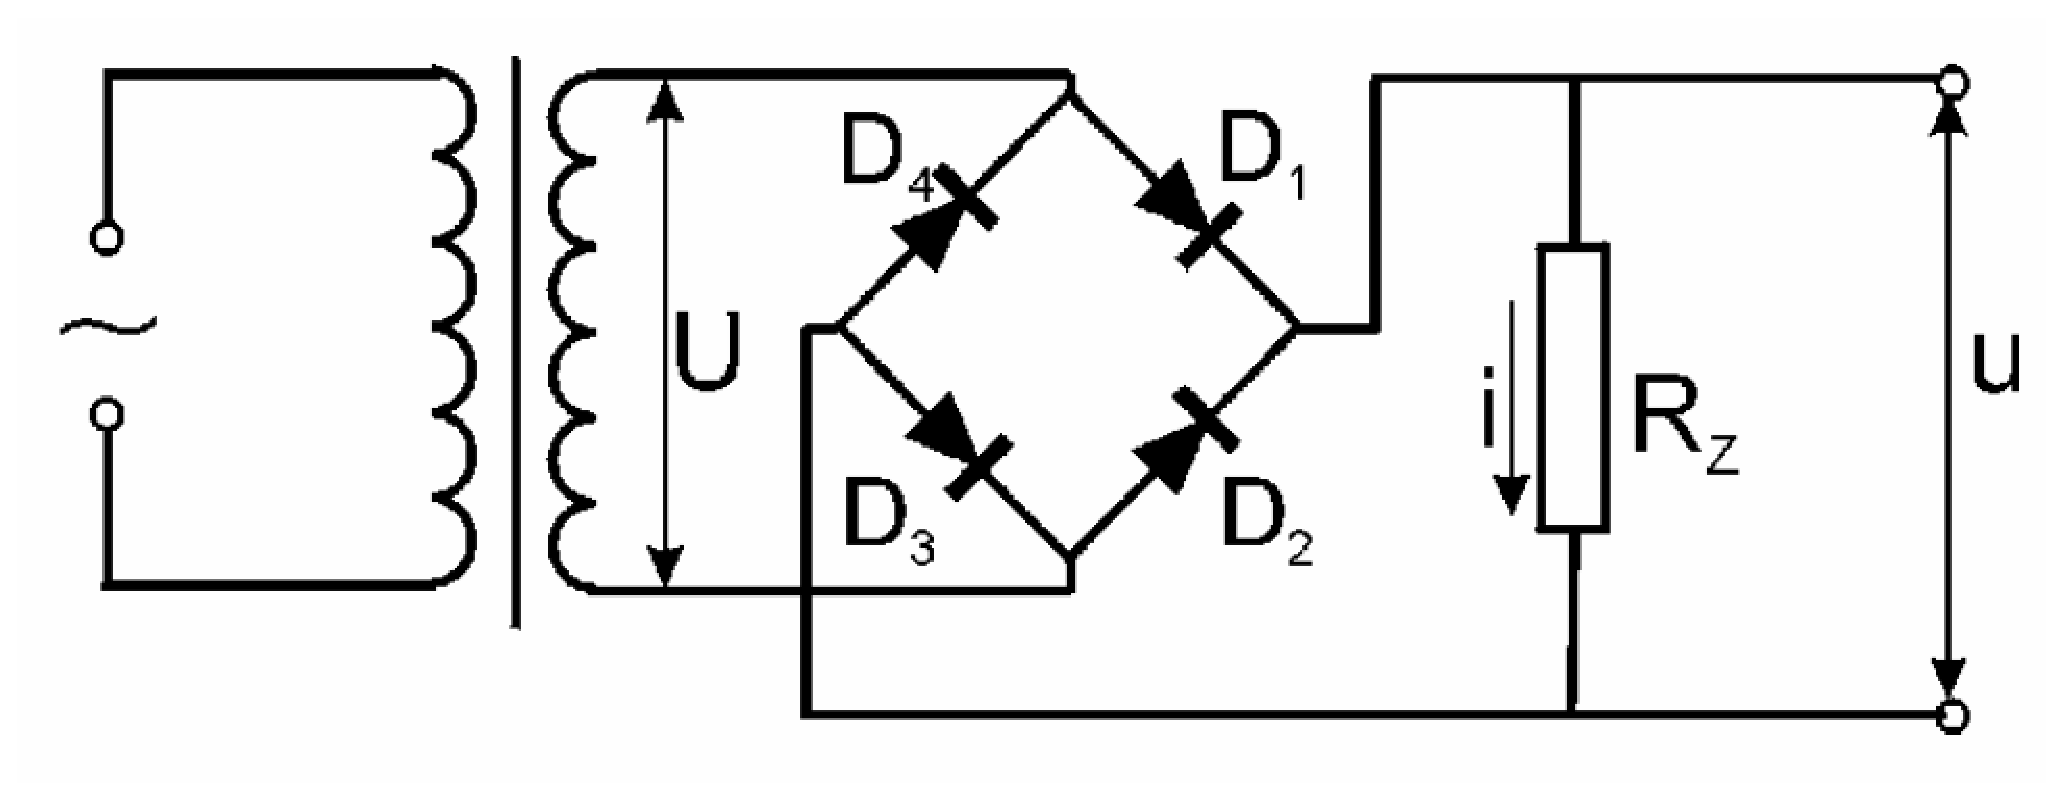
\includegraphics[width=6in]{sch1.eps}
\caption{Schéma zapojení Graetzova můstku.}
\label{sch1}
\end{figure}

\begin{figure}
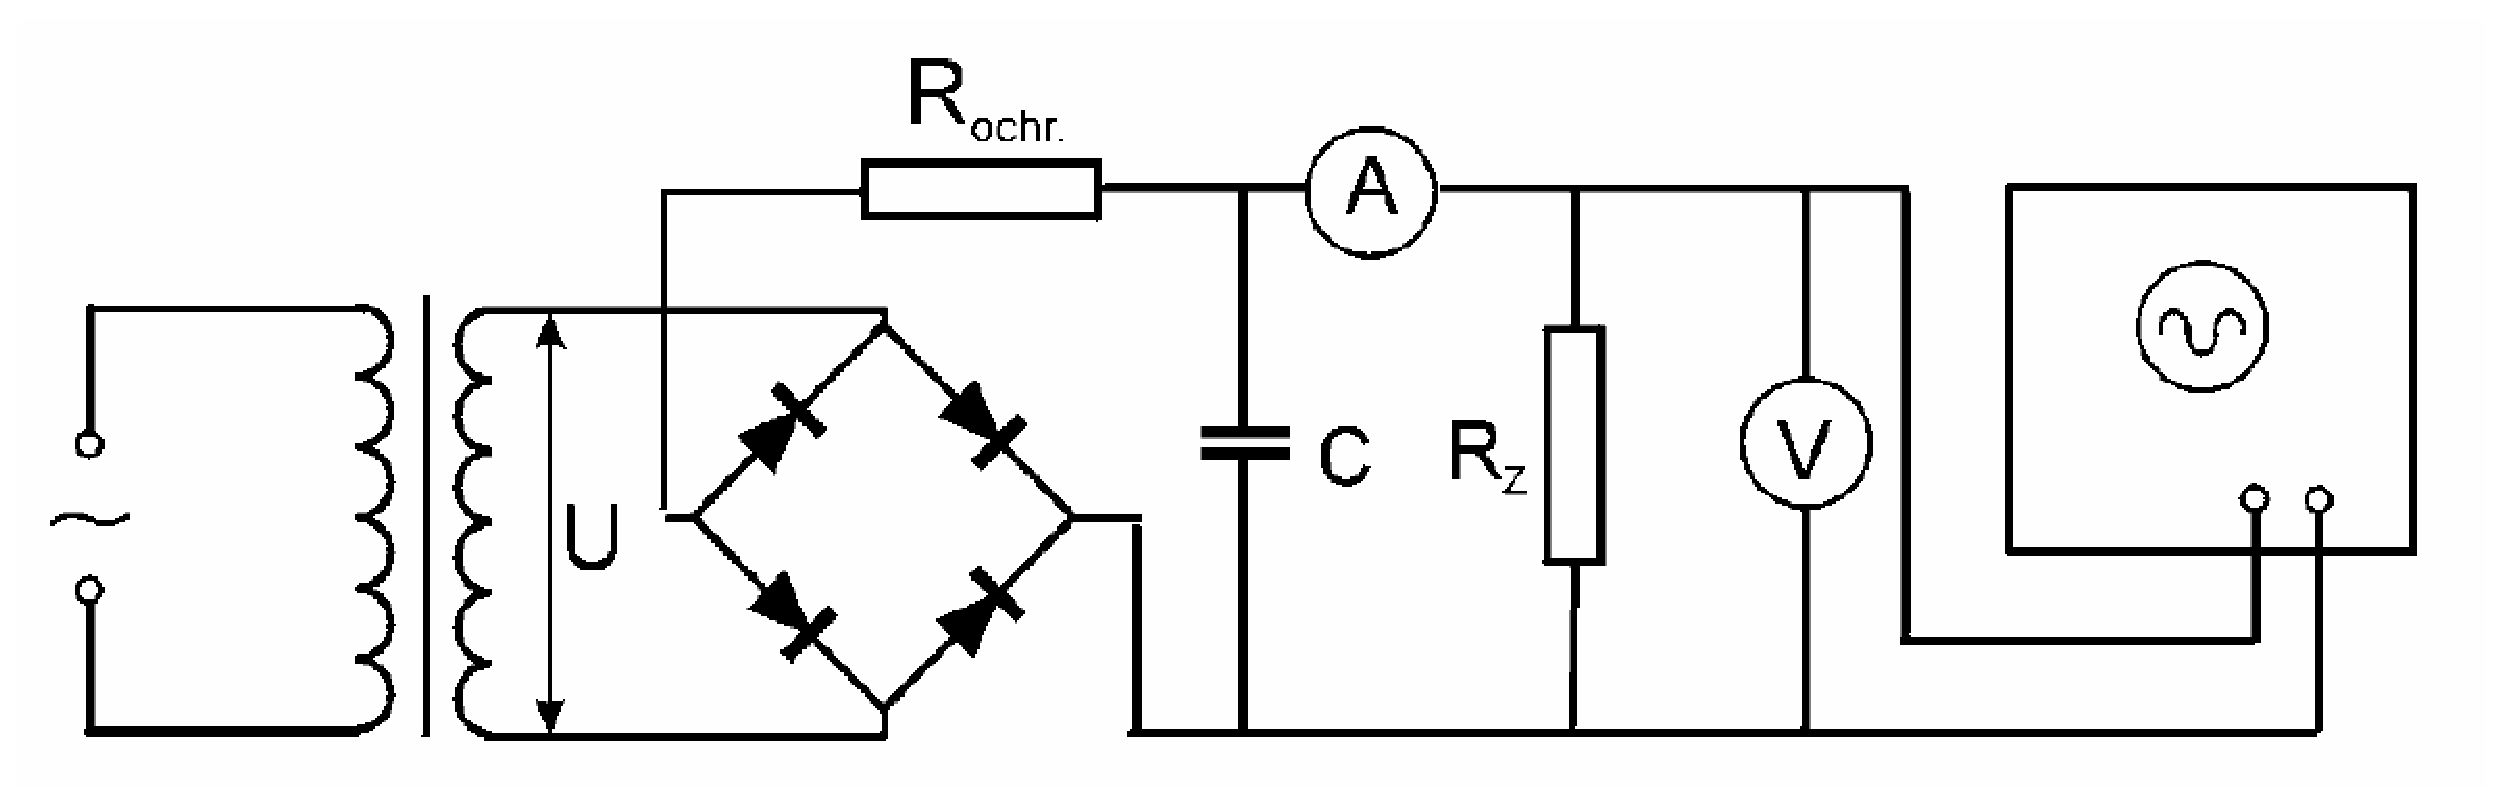
\includegraphics[width=6in]{sch2.eps}
\caption{Schéma pro měření usměrněného rpoudu s filtrční kapacitou.}
\label{sch2}
\end{figure}


\subsection{Graetzův můstek}
Na obrázku (\ref{sch1}) je Graetzův můstek, který se používá jako dvoucestný uměrňovač. Jeho princip je popsán v \cite{text}. 
Pro efektivní hodnotu napětí při tomto zapojení platí
\begin{eqnarray}
U_e=\frac{2}{\pi}U_0.
\label{U_e2}
\end{eqnarray}

\subsection{Filtrace napětí}
Při zapojení dle obrázku (\ref{sch2}) dochází k filtraci napětí. V závislosti na velikosti $C$ a $R_z$ se bude měnit prlběh napětí přibližně dle vztahu
\begin{eqnarray}
u=U_0\left(1-\frac{t}{R_zC}\right).
\end{eqnarray}
Velikost filtrace je popsána veličinou činitel filtrace $k_f$, která je definována vztahem
\begin{eqnarray}
k_f=\frac{U_0}{\Delta U},
\end{eqnarray}
kde $\Delta U$ je špičková hodnota střídavé složky napětí.

V \cite{text} je dále odvozen vztah pro velikost filtrační kapacity
\begin{eqnarray}
C=Tk_fI\cdot(nU_0)^{-1},
\end{eqnarray}
kde $n$ je pro případ dvoucestného usměrnění roven dvěma.

\section{Měření}

\subsection{Špičkové napětí}
Nejprve jsem změřil efektivní hodnotu napětí v sekundárním obvodu, která byla 
\begin{eqnarray}
U_e=(6.97 \pm 0.04)\mbox{V}, 
\end{eqnarray}
čemuž by u čistě sinusového proudu odpovídala velikost špičkového napětí 
\begin{eqnarray}
U_0=(9.86 \pm 0.06)\mbox{V}. 
\end{eqnarray}
Na osciloskopu jsem však naměřil hodnotu 
\begin{eqnarray}
U_0=(10.0\pm0.2)\mbox{V}.
\end{eqnarray}

\subsection{Závislost stejnosměrné složky napětí}
Zvolil jsem si dvoucestné uměrnění a sestavil zapojení dle obrázku (\ref{sch2}). Proměřil jsem 
velikost stejnosměrného napětí na velikosti filtrační kapacity při konstantním 
odporu 10 k$\Omega$. Naměřené hodnoty jsou v tabulce \ref{TUe} a výsledná závislost 
je na obrázku (\ref{g1}), kterou jsem pro názornost proložil křivkou. Pro filtrační 
kapacitu 10 $\mu$F byl činitel filtrace
\begin{eqnarray}
k_f=13.43
\end{eqnarray}

\begin{table}
$$
\begin{array}{|c|c|c|c|c|c|c|c|c|c|c|}
\hline
C/\mu\mbox{F}&  0&  0.1&   0.2&   0.3&   0.4&   0.5&   0.6&   0.7&   0.8&   0.9 \\ \hline
U/\mbox{V}&   5.28&   5.41&   5.65&   5.91&   6.17&   6.42&   6.63&   6.78&   6.93&   7.05   \\ \hline \hline
C/\mu\mbox{F}&  1&   2&   3&   4&   5&   6&   7&   8&   9&   10 \\ \hline
U/\mbox{V}&   7.14&   7.66&   7.92&   8.06&   8.17&   8.20&   8.26&   8.29&   8.30&   8.33    \\ \hline
\end{array}
$$
\caption{Velikost stejnosměrné složky napětí $U$ v závislosti na filtrační kapacitě $C$.}
\label{TUe}
\end{table}

\begin{figure}[htb]
\begin{center}
% GNUPLOT: LaTeX picture with Postscript
\begingroup
  \makeatletter
  \providecommand\color[2][]{%
    \GenericError{(gnuplot) \space\space\space\@spaces}{%
      Package color not loaded in conjunction with
      terminal option `colourtext'%
    }{See the gnuplot documentation for explanation.%
    }{Either use 'blacktext' in gnuplot or load the package
      color.sty in LaTeX.}%
    \renewcommand\color[2][]{}%
  }%
  \providecommand\includegraphics[2][]{%
    \GenericError{(gnuplot) \space\space\space\@spaces}{%
      Package graphicx or graphics not loaded%
    }{See the gnuplot documentation for explanation.%
    }{The gnuplot epslatex terminal needs graphicx.sty or graphics.sty.}%
    \renewcommand\includegraphics[2][]{}%
  }%
  \providecommand\rotatebox[2]{#2}%
  \@ifundefined{ifGPcolor}{%
    \newif\ifGPcolor
    \GPcolorfalse
  }{}%
  \@ifundefined{ifGPblacktext}{%
    \newif\ifGPblacktext
    \GPblacktexttrue
  }{}%
  % define a \g@addto@macro without @ in the name:
  \let\gplgaddtomacro\g@addto@macro
  % define empty templates for all commands taking text:
  \gdef\gplbacktext{}%
  \gdef\gplfronttext{}%
  \makeatother
  \ifGPblacktext
    % no textcolor at all
    \def\colorrgb#1{}%
    \def\colorgray#1{}%
  \else
    % gray or color?
    \ifGPcolor
      \def\colorrgb#1{\color[rgb]{#1}}%
      \def\colorgray#1{\color[gray]{#1}}%
      \expandafter\def\csname LTw\endcsname{\color{white}}%
      \expandafter\def\csname LTb\endcsname{\color{black}}%
      \expandafter\def\csname LTa\endcsname{\color{black}}%
      \expandafter\def\csname LT0\endcsname{\color[rgb]{1,0,0}}%
      \expandafter\def\csname LT1\endcsname{\color[rgb]{0,1,0}}%
      \expandafter\def\csname LT2\endcsname{\color[rgb]{0,0,1}}%
      \expandafter\def\csname LT3\endcsname{\color[rgb]{1,0,1}}%
      \expandafter\def\csname LT4\endcsname{\color[rgb]{0,1,1}}%
      \expandafter\def\csname LT5\endcsname{\color[rgb]{1,1,0}}%
      \expandafter\def\csname LT6\endcsname{\color[rgb]{0,0,0}}%
      \expandafter\def\csname LT7\endcsname{\color[rgb]{1,0.3,0}}%
      \expandafter\def\csname LT8\endcsname{\color[rgb]{0.5,0.5,0.5}}%
    \else
      % gray
      \def\colorrgb#1{\color{black}}%
      \def\colorgray#1{\color[gray]{#1}}%
      \expandafter\def\csname LTw\endcsname{\color{white}}%
      \expandafter\def\csname LTb\endcsname{\color{black}}%
      \expandafter\def\csname LTa\endcsname{\color{black}}%
      \expandafter\def\csname LT0\endcsname{\color{black}}%
      \expandafter\def\csname LT1\endcsname{\color{black}}%
      \expandafter\def\csname LT2\endcsname{\color{black}}%
      \expandafter\def\csname LT3\endcsname{\color{black}}%
      \expandafter\def\csname LT4\endcsname{\color{black}}%
      \expandafter\def\csname LT5\endcsname{\color{black}}%
      \expandafter\def\csname LT6\endcsname{\color{black}}%
      \expandafter\def\csname LT7\endcsname{\color{black}}%
      \expandafter\def\csname LT8\endcsname{\color{black}}%
    \fi
  \fi
  \setlength{\unitlength}{0.0500bp}%
  \begin{picture}(7200.00,5040.00)%
    \gplgaddtomacro\gplbacktext{%
      \csname LTb\endcsname%
      \put(1210,704){\makebox(0,0)[r]{\strut{} 700}}%
      \put(1210,1074){\makebox(0,0)[r]{\strut{} 800}}%
      \put(1210,1444){\makebox(0,0)[r]{\strut{} 900}}%
      \put(1210,1814){\makebox(0,0)[r]{\strut{} 1000}}%
      \put(1210,2184){\makebox(0,0)[r]{\strut{} 1100}}%
      \put(1210,2554){\makebox(0,0)[r]{\strut{} 1200}}%
      \put(1210,2925){\makebox(0,0)[r]{\strut{} 1300}}%
      \put(1210,3295){\makebox(0,0)[r]{\strut{} 1400}}%
      \put(1210,3665){\makebox(0,0)[r]{\strut{} 1500}}%
      \put(1210,4035){\makebox(0,0)[r]{\strut{} 1600}}%
      \put(1210,4405){\makebox(0,0)[r]{\strut{} 1700}}%
      \put(1210,4775){\makebox(0,0)[r]{\strut{} 1800}}%
      \put(1342,484){\makebox(0,0){\strut{} 0}}%
      \put(2263,484){\makebox(0,0){\strut{} 0.5}}%
      \put(3184,484){\makebox(0,0){\strut{} 1}}%
      \put(4105,484){\makebox(0,0){\strut{} 1.5}}%
      \put(5027,484){\makebox(0,0){\strut{} 2}}%
      \put(5948,484){\makebox(0,0){\strut{} 2.5}}%
      \put(6869,484){\makebox(0,0){\strut{} 3}}%
      \put(308,2739){\rotatebox{-270}{\makebox(0,0){\strut{}$h$/keV$\cdot$m$^{-1}$}}}%
      \put(4105,154){\makebox(0,0){\strut{}$x$/cm}}%
    }%
    \gplgaddtomacro\gplfronttext{%
    }%
    \gplbacktext
    \put(0,0){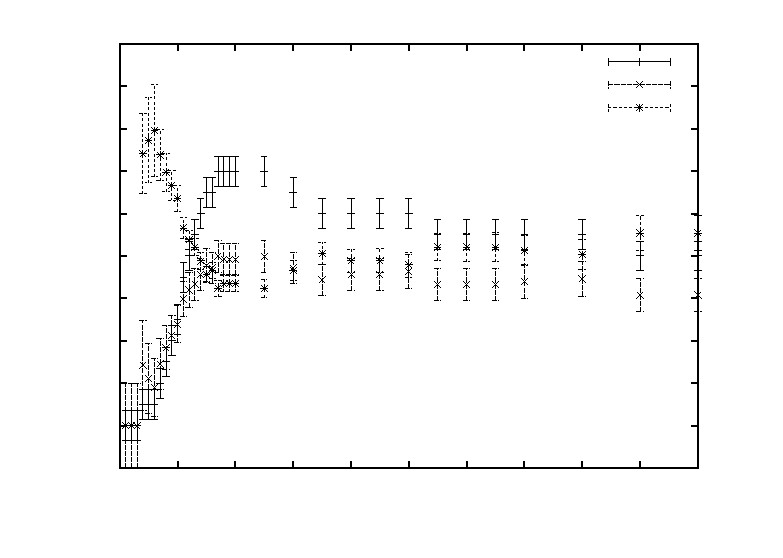
\includegraphics{g1}}%
    \gplfronttext
  \end{picture}%
\endgroup

\end{center}
\caption{Graf závislosti stejnosměrné složky napětí $U$ na velikosti filtrační kapacity $C$.}
\label{g1}
\end{figure}

\subsection{Závislost filtrační kapacity}
Následně jsem měřil potřebnou filtrační kapacitu pro různé proudy, aby $\Delta U=1$V. Tyto 
hodnoty jsou i s potřebným $R_z$ uvedeny v tabulce \ref{TI} a zaneseny do obrázku (\ref{g2}) 
spolu s závislostí časové konstanty $\tau$.

\begin{table}
$$
\begin{array}{|c|c|c|}
\hline
I/\mbox{mA}&    C/\mu\mbox{F}&  R_z/\mbox{k}\Omega \\ \hline
0.10\pm 0.01&    0.86&  70.0\pm0.7 \\ \hline
0.20\pm 0.01&    1.7&   38.5\pm0.4 \\ \hline
0.30\pm 0.01&    2.4&   26.5\pm0.3 \\ \hline
0.40\pm 0.01&    3.2&   19.8\pm0.2 \\ \hline
0.50\pm 0.01&    4.0&   15.8\pm0.2 \\ \hline
0.62\pm 0.01&    4.7&   13.0\pm0.1 \\ \hline
0.68\pm 0.02&    5.1&   12.0\pm0.1 \\ \hline
0.72\pm 0.02&    5.5&   11.2\pm0.1 \\ \hline
0.80\pm 0.02&    6.1&   10.0\pm0.1 \\ \hline
0.86\pm 0.02&    6.6&   9.40\pm0.09 \\ \hline
0.90\pm 0.02&    6.8&   9.00\pm0.09 \\ \hline
0.96\pm 0.02&    7.4&   8.40\pm0.08 \\ \hline
1.00\pm 0.02&    7.6&   8.10\pm0.08 \\ \hline
\end{array}
$$
\caption{Závislosti filtrační kapacity $C$ a odporu $R_z$ na proudu $I$.}
\label{TI}
\end{table}

\begin{figure}
\begin{center}
% GNUPLOT: LaTeX picture with Postscript
\begingroup
  \makeatletter
  \providecommand\color[2][]{%
    \GenericError{(gnuplot) \space\space\space\@spaces}{%
      Package color not loaded in conjunction with
      terminal option `colourtext'%
    }{See the gnuplot documentation for explanation.%
    }{Either use 'blacktext' in gnuplot or load the package
      color.sty in LaTeX.}%
    \renewcommand\color[2][]{}%
  }%
  \providecommand\includegraphics[2][]{%
    \GenericError{(gnuplot) \space\space\space\@spaces}{%
      Package graphicx or graphics not loaded%
    }{See the gnuplot documentation for explanation.%
    }{The gnuplot epslatex terminal needs graphicx.sty or graphics.sty.}%
    \renewcommand\includegraphics[2][]{}%
  }%
  \providecommand\rotatebox[2]{#2}%
  \@ifundefined{ifGPcolor}{%
    \newif\ifGPcolor
    \GPcolorfalse
  }{}%
  \@ifundefined{ifGPblacktext}{%
    \newif\ifGPblacktext
    \GPblacktexttrue
  }{}%
  % define a \g@addto@macro without @ in the name:
  \let\gplgaddtomacro\g@addto@macro
  % define empty templates for all commands taking text:
  \gdef\gplbacktext{}%
  \gdef\gplfronttext{}%
  \makeatother
  \ifGPblacktext
    % no textcolor at all
    \def\colorrgb#1{}%
    \def\colorgray#1{}%
  \else
    % gray or color?
    \ifGPcolor
      \def\colorrgb#1{\color[rgb]{#1}}%
      \def\colorgray#1{\color[gray]{#1}}%
      \expandafter\def\csname LTw\endcsname{\color{white}}%
      \expandafter\def\csname LTb\endcsname{\color{black}}%
      \expandafter\def\csname LTa\endcsname{\color{black}}%
      \expandafter\def\csname LT0\endcsname{\color[rgb]{1,0,0}}%
      \expandafter\def\csname LT1\endcsname{\color[rgb]{0,1,0}}%
      \expandafter\def\csname LT2\endcsname{\color[rgb]{0,0,1}}%
      \expandafter\def\csname LT3\endcsname{\color[rgb]{1,0,1}}%
      \expandafter\def\csname LT4\endcsname{\color[rgb]{0,1,1}}%
      \expandafter\def\csname LT5\endcsname{\color[rgb]{1,1,0}}%
      \expandafter\def\csname LT6\endcsname{\color[rgb]{0,0,0}}%
      \expandafter\def\csname LT7\endcsname{\color[rgb]{1,0.3,0}}%
      \expandafter\def\csname LT8\endcsname{\color[rgb]{0.5,0.5,0.5}}%
    \else
      % gray
      \def\colorrgb#1{\color{black}}%
      \def\colorgray#1{\color[gray]{#1}}%
      \expandafter\def\csname LTw\endcsname{\color{white}}%
      \expandafter\def\csname LTb\endcsname{\color{black}}%
      \expandafter\def\csname LTa\endcsname{\color{black}}%
      \expandafter\def\csname LT0\endcsname{\color{black}}%
      \expandafter\def\csname LT1\endcsname{\color{black}}%
      \expandafter\def\csname LT2\endcsname{\color{black}}%
      \expandafter\def\csname LT3\endcsname{\color{black}}%
      \expandafter\def\csname LT4\endcsname{\color{black}}%
      \expandafter\def\csname LT5\endcsname{\color{black}}%
      \expandafter\def\csname LT6\endcsname{\color{black}}%
      \expandafter\def\csname LT7\endcsname{\color{black}}%
      \expandafter\def\csname LT8\endcsname{\color{black}}%
    \fi
  \fi
  \setlength{\unitlength}{0.0500bp}%
  \begin{picture}(7200.00,5040.00)%
    \gplgaddtomacro\gplbacktext{%
      \csname LTb\endcsname%
      \put(814,704){\makebox(0,0)[r]{\strut{} 0}}%
      \put(814,1213){\makebox(0,0)[r]{\strut{} 1}}%
      \put(814,1722){\makebox(0,0)[r]{\strut{} 2}}%
      \put(814,2231){\makebox(0,0)[r]{\strut{} 3}}%
      \put(814,2740){\makebox(0,0)[r]{\strut{} 4}}%
      \put(814,3248){\makebox(0,0)[r]{\strut{} 5}}%
      \put(814,3757){\makebox(0,0)[r]{\strut{} 6}}%
      \put(814,4266){\makebox(0,0)[r]{\strut{} 7}}%
      \put(814,4775){\makebox(0,0)[r]{\strut{} 8}}%
      \put(946,484){\makebox(0,0){\strut{} 0}}%
      \put(1404,484){\makebox(0,0){\strut{} 0.1}}%
      \put(1863,484){\makebox(0,0){\strut{} 0.2}}%
      \put(2321,484){\makebox(0,0){\strut{} 0.3}}%
      \put(2780,484){\makebox(0,0){\strut{} 0.4}}%
      \put(3238,484){\makebox(0,0){\strut{} 0.5}}%
      \put(3697,484){\makebox(0,0){\strut{} 0.6}}%
      \put(4155,484){\makebox(0,0){\strut{} 0.7}}%
      \put(4614,484){\makebox(0,0){\strut{} 0.8}}%
      \put(5072,484){\makebox(0,0){\strut{} 0.9}}%
      \put(5531,484){\makebox(0,0){\strut{} 1}}%
      \put(5989,484){\makebox(0,0){\strut{} 1.1}}%
      \put(6121,1043){\makebox(0,0)[l]{\strut{} 56}}%
      \put(6121,1722){\makebox(0,0)[l]{\strut{} 58}}%
      \put(6121,2400){\makebox(0,0)[l]{\strut{} 60}}%
      \put(6121,3079){\makebox(0,0)[l]{\strut{} 62}}%
      \put(6121,3757){\makebox(0,0)[l]{\strut{} 64}}%
      \put(6121,4436){\makebox(0,0)[l]{\strut{} 66}}%
      \put(308,2739){\rotatebox{-270}{\makebox(0,0){\strut{}$C/\mu$F}}}%
      \put(6758,2739){\rotatebox{-270}{\makebox(0,0){\strut{}$\tau/$s}}}%
      \put(3467,154){\makebox(0,0){\strut{}$I/$mA}}%
    }%
    \gplgaddtomacro\gplfronttext{%
      \csname LTb\endcsname%
      \put(5002,1317){\makebox(0,0)[r]{\strut{}$C$}}%
      \csname LTb\endcsname%
      \put(5002,1097){\makebox(0,0)[r]{\strut{}$7.72\cdot10^{-3}\{I\}$}}%
      \csname LTb\endcsname%
      \put(5002,877){\makebox(0,0)[r]{\strut{}$\tau$}}%
    }%
    \gplbacktext
    \put(0,0){\includegraphics{g2}}%
    \gplfronttext
  \end{picture}%
\endgroup

\end{center}
\caption{Graf závislosti filtrační kapacity $C$ a časové konstanty $\tau$ na proudu $I$.}
\label{g2}
\end{figure}

\subsection{Dioda}
Za pomoci osciloskopu proměřil VA charakteristiku diody. Klíčové body jsou v tabulce 
\ref{TDioda} a výsledná charakteristika je na obrázku (\ref{g3}). Nebylo možné stanovit přesnou 
chybu měření, protože na osciloskopu vznikaly dvě křivky a i při postupu po bodech byla špička 
křivky těžko určitelná. Při proudu 20 mA by mělo na diodě být napětí asi 60.6 V.

\begin{table}
$$
\begin{array}{|c|c|}
\hline
U/\mbox{V}& I/\mbox{mA} \\ \hline
<-0.6&  0 \\ \hline
0&  1 \\ \hline
0.4&    2 \\ \hline
0.8&    3 \\ \hline
1.8&    6 \\ \hline
\end{array}
$$
\caption{Klíčové hodnoty VA charakteristiky diody}
\label{TDioda}
\end{table}

\begin{figure}
\begin{center}
% GNUPLOT: LaTeX picture with Postscript
\begingroup
  \makeatletter
  \providecommand\color[2][]{%
    \GenericError{(gnuplot) \space\space\space\@spaces}{%
      Package color not loaded in conjunction with
      terminal option `colourtext'%
    }{See the gnuplot documentation for explanation.%
    }{Either use 'blacktext' in gnuplot or load the package
      color.sty in LaTeX.}%
    \renewcommand\color[2][]{}%
  }%
  \providecommand\includegraphics[2][]{%
    \GenericError{(gnuplot) \space\space\space\@spaces}{%
      Package graphicx or graphics not loaded%
    }{See the gnuplot documentation for explanation.%
    }{The gnuplot epslatex terminal needs graphicx.sty or graphics.sty.}%
    \renewcommand\includegraphics[2][]{}%
  }%
  \providecommand\rotatebox[2]{#2}%
  \@ifundefined{ifGPcolor}{%
    \newif\ifGPcolor
    \GPcolorfalse
  }{}%
  \@ifundefined{ifGPblacktext}{%
    \newif\ifGPblacktext
    \GPblacktexttrue
  }{}%
  % define a \g@addto@macro without @ in the name:
  \let\gplgaddtomacro\g@addto@macro
  % define empty templates for all commands taking text:
  \gdef\gplbacktext{}%
  \gdef\gplfronttext{}%
  \makeatother
  \ifGPblacktext
    % no textcolor at all
    \def\colorrgb#1{}%
    \def\colorgray#1{}%
  \else
    % gray or color?
    \ifGPcolor
      \def\colorrgb#1{\color[rgb]{#1}}%
      \def\colorgray#1{\color[gray]{#1}}%
      \expandafter\def\csname LTw\endcsname{\color{white}}%
      \expandafter\def\csname LTb\endcsname{\color{black}}%
      \expandafter\def\csname LTa\endcsname{\color{black}}%
      \expandafter\def\csname LT0\endcsname{\color[rgb]{1,0,0}}%
      \expandafter\def\csname LT1\endcsname{\color[rgb]{0,1,0}}%
      \expandafter\def\csname LT2\endcsname{\color[rgb]{0,0,1}}%
      \expandafter\def\csname LT3\endcsname{\color[rgb]{1,0,1}}%
      \expandafter\def\csname LT4\endcsname{\color[rgb]{0,1,1}}%
      \expandafter\def\csname LT5\endcsname{\color[rgb]{1,1,0}}%
      \expandafter\def\csname LT6\endcsname{\color[rgb]{0,0,0}}%
      \expandafter\def\csname LT7\endcsname{\color[rgb]{1,0.3,0}}%
      \expandafter\def\csname LT8\endcsname{\color[rgb]{0.5,0.5,0.5}}%
    \else
      % gray
      \def\colorrgb#1{\color{black}}%
      \def\colorgray#1{\color[gray]{#1}}%
      \expandafter\def\csname LTw\endcsname{\color{white}}%
      \expandafter\def\csname LTb\endcsname{\color{black}}%
      \expandafter\def\csname LTa\endcsname{\color{black}}%
      \expandafter\def\csname LT0\endcsname{\color{black}}%
      \expandafter\def\csname LT1\endcsname{\color{black}}%
      \expandafter\def\csname LT2\endcsname{\color{black}}%
      \expandafter\def\csname LT3\endcsname{\color{black}}%
      \expandafter\def\csname LT4\endcsname{\color{black}}%
      \expandafter\def\csname LT5\endcsname{\color{black}}%
      \expandafter\def\csname LT6\endcsname{\color{black}}%
      \expandafter\def\csname LT7\endcsname{\color{black}}%
      \expandafter\def\csname LT8\endcsname{\color{black}}%
    \fi
  \fi
  \setlength{\unitlength}{0.0500bp}%
  \begin{picture}(7200.00,5040.00)%
    \gplgaddtomacro\gplbacktext{%
      \csname LTb\endcsname%
      \put(1210,704){\makebox(0,0)[r]{\strut{} 0}}%
      \put(1210,1382){\makebox(0,0)[r]{\strut{} 500}}%
      \put(1210,2061){\makebox(0,0)[r]{\strut{} 1000}}%
      \put(1210,2739){\makebox(0,0)[r]{\strut{} 1500}}%
      \put(1210,3418){\makebox(0,0)[r]{\strut{} 2000}}%
      \put(1210,4096){\makebox(0,0)[r]{\strut{} 2500}}%
      \put(1210,4775){\makebox(0,0)[r]{\strut{} 3000}}%
      \put(1342,484){\makebox(0,0){\strut{} 30}}%
      \put(1956,484){\makebox(0,0){\strut{} 40}}%
      \put(2570,484){\makebox(0,0){\strut{} 50}}%
      \put(3184,484){\makebox(0,0){\strut{} 60}}%
      \put(3798,484){\makebox(0,0){\strut{} 70}}%
      \put(4413,484){\makebox(0,0){\strut{} 80}}%
      \put(5027,484){\makebox(0,0){\strut{} 90}}%
      \put(5641,484){\makebox(0,0){\strut{} 100}}%
      \put(6255,484){\makebox(0,0){\strut{} 110}}%
      \put(6869,484){\makebox(0,0){\strut{} 120}}%
      \put(308,2739){\rotatebox{-270}{\makebox(0,0){\strut{}$f$/Hz}}}%
      \put(4105,154){\makebox(0,0){\strut{}$U_0$/V}}%
    }%
    \gplgaddtomacro\gplfronttext{%
    }%
    \gplbacktext
    \put(0,0){\includegraphics{g3}}%
    \gplfronttext
  \end{picture}%
\endgroup

\end{center}
\caption{VA charakteristika diody}
\label{g3}
\end{figure}

\subsection{Zenerova dioda}
Stejný postup jako u diody jsem zvolil u Zenerovy diody. Klíčové body jsou v tabulce \ref{TZener} 
a výsledná charakteristika na obrázku (\ref{g4}). Při proudu 20 mA bylo na Zenerově diodě přibližně 0.64 V a Zenerovo napětí je přibližně -6.2 V.

\begin{table}
$$
\begin{array}{|c|c|}
\hline
U/\mbox{V}& I/\mbox{mA} \\ \hline
-6.6&  -15 \\ \hline
-6.5&  -10 \\ \hline
-6.4&    -5 \\ \hline
-6.2&    0 \\ \hline
0.4&    0 \\ \hline
0.64&    20 \\ \hline
0.66&    40 \\ \hline
0.68&    60 \\ \hline
\end{array}
$$
\caption{Klíčové hodnoty VA charakteristiky Zenerovy diody}
\label{TZener}
\end{table}

\begin{figure}
\begin{center}
% GNUPLOT: LaTeX picture with Postscript
\begingroup
  \makeatletter
  \providecommand\color[2][]{%
    \GenericError{(gnuplot) \space\space\space\@spaces}{%
      Package color not loaded in conjunction with
      terminal option `colourtext'%
    }{See the gnuplot documentation for explanation.%
    }{Either use 'blacktext' in gnuplot or load the package
      color.sty in LaTeX.}%
    \renewcommand\color[2][]{}%
  }%
  \providecommand\includegraphics[2][]{%
    \GenericError{(gnuplot) \space\space\space\@spaces}{%
      Package graphicx or graphics not loaded%
    }{See the gnuplot documentation for explanation.%
    }{The gnuplot epslatex terminal needs graphicx.sty or graphics.sty.}%
    \renewcommand\includegraphics[2][]{}%
  }%
  \providecommand\rotatebox[2]{#2}%
  \@ifundefined{ifGPcolor}{%
    \newif\ifGPcolor
    \GPcolorfalse
  }{}%
  \@ifundefined{ifGPblacktext}{%
    \newif\ifGPblacktext
    \GPblacktexttrue
  }{}%
  % define a \g@addto@macro without @ in the name:
  \let\gplgaddtomacro\g@addto@macro
  % define empty templates for all commands taking text:
  \gdef\gplbacktext{}%
  \gdef\gplfronttext{}%
  \makeatother
  \ifGPblacktext
    % no textcolor at all
    \def\colorrgb#1{}%
    \def\colorgray#1{}%
  \else
    % gray or color?
    \ifGPcolor
      \def\colorrgb#1{\color[rgb]{#1}}%
      \def\colorgray#1{\color[gray]{#1}}%
      \expandafter\def\csname LTw\endcsname{\color{white}}%
      \expandafter\def\csname LTb\endcsname{\color{black}}%
      \expandafter\def\csname LTa\endcsname{\color{black}}%
      \expandafter\def\csname LT0\endcsname{\color[rgb]{1,0,0}}%
      \expandafter\def\csname LT1\endcsname{\color[rgb]{0,1,0}}%
      \expandafter\def\csname LT2\endcsname{\color[rgb]{0,0,1}}%
      \expandafter\def\csname LT3\endcsname{\color[rgb]{1,0,1}}%
      \expandafter\def\csname LT4\endcsname{\color[rgb]{0,1,1}}%
      \expandafter\def\csname LT5\endcsname{\color[rgb]{1,1,0}}%
      \expandafter\def\csname LT6\endcsname{\color[rgb]{0,0,0}}%
      \expandafter\def\csname LT7\endcsname{\color[rgb]{1,0.3,0}}%
      \expandafter\def\csname LT8\endcsname{\color[rgb]{0.5,0.5,0.5}}%
    \else
      % gray
      \def\colorrgb#1{\color{black}}%
      \def\colorgray#1{\color[gray]{#1}}%
      \expandafter\def\csname LTw\endcsname{\color{white}}%
      \expandafter\def\csname LTb\endcsname{\color{black}}%
      \expandafter\def\csname LTa\endcsname{\color{black}}%
      \expandafter\def\csname LT0\endcsname{\color{black}}%
      \expandafter\def\csname LT1\endcsname{\color{black}}%
      \expandafter\def\csname LT2\endcsname{\color{black}}%
      \expandafter\def\csname LT3\endcsname{\color{black}}%
      \expandafter\def\csname LT4\endcsname{\color{black}}%
      \expandafter\def\csname LT5\endcsname{\color{black}}%
      \expandafter\def\csname LT6\endcsname{\color{black}}%
      \expandafter\def\csname LT7\endcsname{\color{black}}%
      \expandafter\def\csname LT8\endcsname{\color{black}}%
    \fi
  \fi
  \setlength{\unitlength}{0.0500bp}%
  \begin{picture}(7200.00,5040.00)%
    \gplgaddtomacro\gplbacktext{%
      \csname LTb\endcsname%
      \put(1210,704){\makebox(0,0)[r]{\strut{} 900}}%
      \put(1210,1383){\makebox(0,0)[r]{\strut{} 950}}%
      \put(1210,2061){\makebox(0,0)[r]{\strut{} 1000}}%
      \put(1210,2740){\makebox(0,0)[r]{\strut{} 1050}}%
      \put(1210,3418){\makebox(0,0)[r]{\strut{} 1100}}%
      \put(1210,4097){\makebox(0,0)[r]{\strut{} 1150}}%
      \put(1210,4775){\makebox(0,0)[r]{\strut{} 1200}}%
      \put(1342,484){\makebox(0,0){\strut{} 2}}%
      \put(2263,484){\makebox(0,0){\strut{} 3}}%
      \put(3184,484){\makebox(0,0){\strut{} 4}}%
      \put(4105,484){\makebox(0,0){\strut{} 5}}%
      \put(5027,484){\makebox(0,0){\strut{} 6}}%
      \put(5948,484){\makebox(0,0){\strut{} 7}}%
      \put(6869,484){\makebox(0,0){\strut{} 8}}%
      \put(308,2739){\rotatebox{-270}{\makebox(0,0){\strut{}$H$/Am$^-1$}}}%
      \put(4105,154){\makebox(0,0){\strut{}$x$/cm}}%
    }%
    \gplgaddtomacro\gplfronttext{%
      \csname LTb\endcsname%
      \put(5882,4602){\makebox(0,0)[r]{\strut{}teoretická}}%
      \csname LTb\endcsname%
      \put(5882,4382){\makebox(0,0)[r]{\strut{}fitovaná}}%
    }%
    \gplbacktext
    \put(0,0){\includegraphics{g4}}%
    \gplfronttext
  \end{picture}%
\endgroup

\end{center}
\caption{VA charakteristika Zenerovy diody}
\label{g4}
\end{figure}

\section{Diskuze}

Proud v sekundárním obvodu nemá čistě sinuový charakter. To bylo nejlépe vidět na jeho prlběhu 
zobrazeném na osciloskopu. Z toho důvodu efektivní a špičová hodnota napětí nesplňuje zcela 
přesně vztah \ref{U_e}.

Závislost stejnosměrné složky napětí na filtrační kapacitě jasně splňujě exponenciální závslost. 
Při maximální filtrační kapacitě byl činitel filtrace vysoký a výsledný proud již měl témeř 
stejnosměrný charakter.

Závislost filtrační kapacity na proudu v sekundárním obvodu vyšla dle předpokladu lineární, a to 
dokonce s velmi malou chybou fitu. Závislost časové konstanty již měla jistou odchylku u nižších 
hodnot proudum která byla zřejmě způsobena vyšší chybou na odporové dekádě.

Charakteristiky diod jsou podle mého jen přibližné, ač vystihují charakter těchto součástek. 
Naměřené hodnoty totiž mají značnou chybu způsobenou rozdvojením křivky na oscilskopu. 

\section{Závěr}
\noindent
Za pomoci osciloskopu jsem stanovil hodnotu špičkového napětí v sekundárním obvodu
\begin{eqnarray}
U=(10.0\pm0.2)\mbox{V}
\end{eqnarray}
a porovnal jí s hodnotou odpovídající výpočtu z voltmetru, která byla
\begin{eqnarray}
U=(9.86\pm0.06)\mbox{V}.
\end{eqnarray}
Proměřil jsem závislost stejnosměré složky proudu na filtrační kapacitě pro proud uměrnění za 
pomoci Graetzova můstku. Naměřené hodnoty jsou v tabulce \ref{TUe} a závislost na obrázku 
\ref{g1}. Hodnotu špičkového napětí jsem porovnou s hodnotou pulzního průběhu. Výsledný činitel 
filtrace byl
\begin{eqnarray}
k_f=13.43
\end{eqnarray}
Proměřil jsem závislost filtrační kapacity na proudu. Výsledky jsou v tabulce \ref{TI}. Závislost 
je zobrazena na obrázku \ref{g2} spolu se závislostí časové konstanty $\tau$. \\
Proměřil jsem charakteristiku diody respektive Zenerovy diody. Výsledná VA charakteristika je 
na ovrázku \ref{g3} respektive \ref{g4}.\\
Stanovil jsem hodnoty napětí na diodách při proudu 20 mA
\begin{eqnarray}
U&=&60.6 \mbox{V} ,\mbox{resp.} \\
U&=&0.64 \mbox{V}.
\end{eqnarray}
Stanovil jsem hodnotu Zenerova napětí na
\begin{eqnarray}
U_z=-6.2\mbox{V}
\end{eqnarray}

\begin{thebibliography}{5}
	\bibitem{text} \textbf{Studijní text na praktikum II} \\http://physics.mff.cuni.cz/vyuka/zfp/txt\_205.htm (3. 11. 2011)
    \bibitem{chyba} \emph{J. Englich}: \textbf{Zpracování výsldků fyzikálních měření} \\ LS 1999/2000
\end{thebibliography}
\end{document}
